
%导言区
\documentclass{article}%book,report,letter

\usepackage{ctex}
\usepackage{fontspec}
%\usepackage{color}
%\usepackage{graphicx} %use graph format
%\usepackage{subfigure}
%\usepackage{epstopdf} %eps图片
\usepackage{amsmath}  %字体加粗
%\usepackage{math}
\usepackage{amsthm}
\usepackage{amssymb} %因为所以符号


%制作页眉页脚
\usepackage{fancyhdr}  
\pagestyle{fancy}  
\lhead{第六周作业}  
\chead{微分方程数值解法}  
\rhead{桑明达 15300180062}  
\lfoot{}  
\cfoot{\thepage}  
\rfoot{}  
\renewcommand{\headrulewidth}{0.4pt}  
\renewcommand{\footrulewidth}{0.4pt} 

%标题
\author{names}
\title{\heiti 微分方程数值解法\\ [2ex] \begin{large} 第六周作业 \end{large}}
\author{\kaishu 桑明达 15300180062}
\date{\today}

% 正文区
\begin{document}
\maketitle

%\newpage

\section{P93 1 Adams格式的Newton表示}

\begin{proof}
	关于$ f\left ( t,u \right ) $的Lagrange插值多项式$ q\left ( t \right ) $可以表示为
\begin{align*}
	q\left ( t \right )=& q\left ( t_{n}+s\Delta t \right )=\sum_{j=0}^{k-1}\left (-1  \right )^{j}\binom{-s+1}{j}\bigtriangledown ^{j}f_{n+1} \\
	\therefore u_{n+1}-u_{n} =& \sum_{j=0}^{k}c_j \bigtriangledown ^j f_{n+1} \\
\end{align*}
    其中$c_j= \left (-1  \right )^{n}\int_{t_n}^{t_{n+1}}\binom{-s+1}{j} \mathrm{d} s $
\end{proof}

\section{P93 2 不同的初始选取对精度的影响}

\begin{proof}
	对于标准测试问题,选取$a=-2$、$t_0=0$、$dt=0.1$、$T=1$、$u_0=1$,使用'精确的初始值','EulerExplicit','Runge-Kutta2','Kutta3','Runge-Kutta4'计算前四个初始值,分别用四阶Adams格式和Geer格式进行精度测试,结果分别如图\ref{Fig:1}、图\ref{Fig:2}。
	
	\begin{figure}
		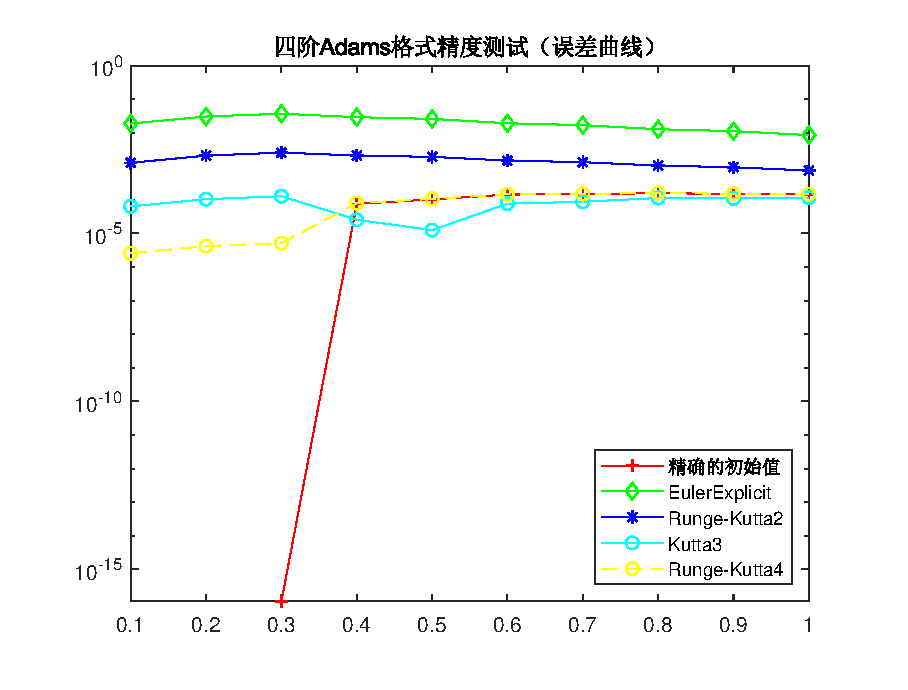
\includegraphics[width=1\linewidth]{week6_2_1.eps}
		\caption{四阶Adams格式}  
		\label{Fig:1}
	\end{figure}

\begin{figure}
	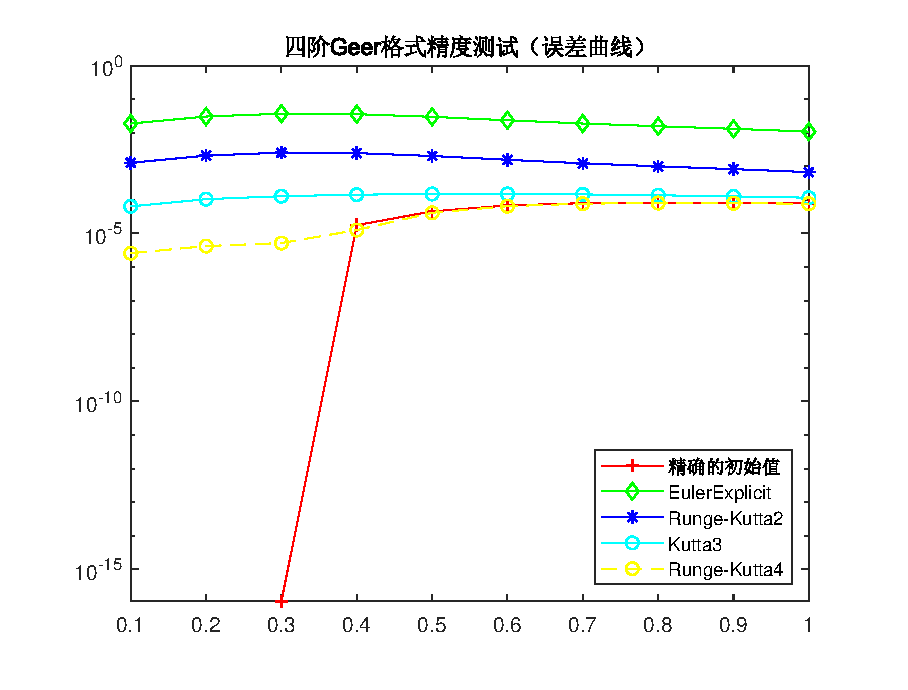
\includegraphics[width=1\linewidth]{week6_2_2.eps}
	\caption{四阶Geer格式}  
	\label{Fig:2}
\end{figure}
	
	
	
\end{proof}

\end{document}